\documentclass{article}

\usepackage{tikz} 
\usetikzlibrary{automata, positioning, arrows} 

\usepackage{amsmath}
\usepackage{amsthm}
\usepackage{amsfonts}
\usepackage{amsmath}
\usepackage{amssymb}
\usepackage{fullpage}
\usepackage{color}
\usepackage{parskip}
\usepackage{graphicx}
\usepackage{hyperref}
  \hypersetup{
    colorlinks = true,
    urlcolor = blue,       % color of external links using \href
    linkcolor= blue,       % color of internal links 
    citecolor= blue,       % color of links to bibliography
    filecolor= blue,        % color of file links
    }
    
\usepackage{listings}

\definecolor{dkgreen}{rgb}{0,0.6,0}
\definecolor{gray}{rgb}{0.5,0.5,0.5}
\definecolor{mauve}{rgb}{0.58,0,0.82}

\lstset{frame=tb,
  language=haskell,
  aboveskip=3mm,
  belowskip=3mm,
  showstringspaces=false,
  columns=flexible,
  basicstyle={\small\ttfamily},
  numbers=none,
  numberstyle=\tiny\color{gray},
  keywordstyle=\color{blue},
  commentstyle=\color{dkgreen},
  stringstyle=\color{mauve},
  breaklines=true,
  breakatwhitespace=true,
  tabsize=3
}

\newtheoremstyle{theorem}
  {\topsep}   % ABOVESPACE
  {\topsep}   % BELOWSPACE
  {\itshape\/}  % BODYFONT
  {0pt}       % INDENT (empty value is the same as 0pt)
  {\bfseries} % HEADFONT
  {.}         % HEADPUNCT
  {5pt plus 1pt minus 1pt} % HEADSPACE
  {}          % CUSTOM-HEAD-SPEC
\theoremstyle{theorem} 
   \newtheorem{theorem}{Theorem}[section]
   \newtheorem{corollary}[theorem]{Corollary}
   \newtheorem{lemma}[theorem]{Lemma}
   \newtheorem{proposition}[theorem]{Proposition}
\theoremstyle{definition}
   \newtheorem{definition}[theorem]{Definition}
   \newtheorem{example}[theorem]{Example}
\theoremstyle{remark}    
  \newtheorem{remark}[theorem]{Remark}

\title{CPSC-354 Report}
\author{Your Name  \\ Chapman University}

\date{\today} 

\begin{document}

\maketitle

\begin{abstract}
If will write this abstract... later!
\end{abstract}

\setcounter{tocdepth}{3}
\tableofcontents

\section{Introduction}\label{intro}

This introduction will be filled later, when I know what I want to say!

Grading  guidelines (see also below):
\begin{itemize}
\item Is typesetting and layout professional? 
\item Is the technical content, in particular the homework, correct?
\item Did the student find interesting references~\cite{bla} and cites them throughout the report?
\item Do the notes reflect understanding and critical thinking?
\item Does the report contain material related to but going beyond what we do in class?
\item Are the questions interesting?
\end{itemize}

Do not change the template (fontsize, width of margin, spacing of lines, etc) without asking your first.

\section{Week by Week}\label{homework}

\subsection{Week 1}

\subsubsection*{Notes}
This week in class we mainly focused on learning Lean, setting up \LaTeX, and a brief lecture on the basis of $Proof = Program$. This idea shows how logical mathematical proofs are a constructive process, building on previously founded theorems and definitions. This idea transfers to theoretical programming in the sense that programs are also constructed proofs. The execution of a program is the execution of many logical steps in a proof. I enjoy how this relates to the "human" process as well - our activities are the execution of previously learned strategies in a logical way.

\subsubsection*{Question} I was interested in learning more about Proof = Program, and some additional sleuthing showed me how a running a program is simply executing the steps in a logical proof. I was wondering how more complex program design methods such as recursion adhere to this idea, and if there are other programming methodologies that do not adhere to Proof = Program?

\subsubsection*{Homework}

  \subsubsection*{Level 5 - Adding Zero}
  In this level we prove the theorem that $\textbf{a+0=a}$ using $\textbf{a+(b+0)+(c+0)=a+b+c}$. Here is how I solved this theorem.

  \bgroup\obeylines
  \qquad \textbf{repeat rw add zero}
  \qquad \textbf{rfl}
  \egroup

  \subsubsection*{Level 6 - Adding Zero}
  In this level we built on the solution from the previous level to learn how to use precision rewriting.

  \bgroup\obeylines
  \qquad \textbf{rw add zero c}
  \qquad \textbf{repeat rw add zero}
  \qquad \textbf{rfl}
  \egroup

  \subsubsection*{Level 7 - Add Suc}
  In this level we prove the theorem that $\textbf{succ(a)=a+1}$.

  \bgroup\obeylines
  \qquad \textbf{rw one eq add zero}
  \qquad \textbf{repeat rw add zero}
  \qquad \textbf{rfl}
  \egroup

  \subsubsection*{Level 8 - Add Suc}
  In this level we prove the equation that $\textbf{2+2=4}$. This was the final level in the Tutorial World, and required the accumulation of definitions and theorems learned so far. I will provide the assumptions that I used when deciding my proof in Lean.

  \bgroup\obeylines
  \qquad \textbf{rw four eq succ three} —— Any number $n = succ(pred(n))$
  \qquad \textbf{rw three eq succ two}  —— Any number $n = succ(pred(n))$
  \qquad \textbf{rw two eq succ one}    —— Any number $n = succ(pred(n))$
  \qquad \textbf{rw one eq succ zero}   —— Any number $n = succ(pred(n))$
  \qquad \textbf{repeat rw add succ}    —— Using $a + succ b = succ (a + b)$
  \qquad \textbf{rw add zero}           —— Using $a + 0 = a$
  \qquad \textbf{rfl}                   —— Proves the goal $X = X$

  \egroup

%In case you want to draw automata in Latex, you can use the tikz %package. Here is an example of a simple automaton:
%
%\begin{tikzpicture}[shorten >=1pt,node distance=2cm,on grid,auto] 
%  \node[state] (q_1)   {$q_1$}; 
%  \node[state] (q_2) [above right=of q_1] {$q_2$}; 
%  \node[state] (q_3) [below right=of q_2] {$q_3$}; 
%   \path[->] 
%   (q_1) edge  node {0} (q_2)
%         edge  node [swap] {1} (q_3)
%   (q_2) edge  node  {1} (q_3)
%         edge [loop above] node {0} ()
%   (q_3) edge [loop below] node {0,1} ();
%\end{tikzpicture}
%
%By the way, GPT-4 is quite good at outputting tikz code.

\subsubsection*{Comments and Questions}

%(Delete and Replace:) Here you should write your own critical reflection on the content of the week. If you can surprise me with something I have not seen before, you are on the right track.

%I expect you to read the lecture notes. 

Ask at least one \textbf{interesting question}\footnote{It is important to learn to ask \emph{interesting} questions. There is no precise way of defining what is meant by interesting. You can only learn this by doing. An interesting question comes typically in two parts. Part 1 (one or two sentences) sets the scene. Part 2 (one or two sentences) asks the question. A good question strikes the right balance between being specific and technical on the one hand and open ended on the other hand. A question that can be answered with yes/no is not an interesing question.} on the lecture notes. Also post the question on the Discord channel so that everybody can see and discuss the questions.

\subsection{Week 2}

\subsubsection*{Notes}
Translating Lean into Math by matching each line in Lean to the corresponding mathematical equation and assumptions. Being able to reverse the proof and translate from Math into Lean is also important. Lean reads from the goal to the axioms, whereas Math is written from the axioms to the goal (usually).
\newline \newline Defining data types recursively (in terms of itself). Syntax varies by language. 
\newline \newline Recursion example with the Tower of Hanoi. Breaking logical puzzles into iterative steps, then into recursive steps.

\subsubsection*{Question}
In class we used recursion to prove an algorithmic solution for the tower of hanoi game. Within the scope of proofs, what are the biggest drawbacks/advantages to using iterative vs recursive techniques?

%(Delete:) Week 2 (and all the other weeks) should follow the same pattern as Week 1. Even if there is a week without homework, notes and comments (see above) are still expected.

\subsubsection*{Homework}

\subsubsection*{Level 1 - Zero Add}
  In this level we prove the theorem that $\textbf{0 + n = n}$. It was our first use of proof by induction.

  \bgroup\obeylines
  \qquad \textbf{induction n with d hd}
  \qquad \textbf{rw add zero}
  \qquad \textbf{rfl}
  \qquad \textbf{rw add succ}
  \qquad \textbf{rw hd}
  \qquad \textbf{rfl}
  \egroup

  \subsubsection*{Level 2 - Succ Add}
  In this level we prove the theorem that $\textbf{succ(a) + b = succ(a + b)}$.

  \bgroup\obeylines
  \qquad \textbf{induction b with d hd}
  \qquad \textbf{repeat rw add zero}
  \qquad \textbf{rfl}
  \qquad \textbf{rw add succ}
  \qquad \textbf{rw hd}
  \qquad \textbf{rw add succ}
  \qquad \textbf{rfl}
  \egroup

  \subsubsection*{Level 3 - Add Comm}
  In this level we prove the theorem that $\textbf{a + b = b + a}$.

  \bgroup\obeylines
  \qquad \textbf{induction b}
  \qquad \textbf{rw add zero}
  \qquad \textbf{rw zero add}
  \qquad \textbf{rfl}
  \qquad \textbf{rw succ add}
  \qquad \textbf{rw add succ}
  \qquad \textbf{rw nih}
  \qquad \textbf{rfl}
  \egroup

  \subsubsection*{Level 4 - Add Assoc}
  In this level we prove the theorem that $\textbf{(a + b) + c = a + (b + c)}$.

  \bgroup\obeylines
  \qquad \textbf{induction b}
  \qquad \textbf{rw add zero}
  \qquad \textbf{rw zero add}
  \qquad \textbf{rfl}
  \qquad \textbf{rw add succ}
  \qquad \textbf{rw succ add}
  \qquad \textbf{rw nih}
  \qquad \textbf{rw add comm}
  \qquad \textbf{rw succ add}
  \qquad \textbf{rw add succ}
  \qquad \textbf{rfl}
  \egroup

  \subsubsection*{Level 5 - Add Comm Right}
  In this level we prove the theorem that $\textbf{(a + b) + c = (a + c) + b}$. I will show the mathematical assumptions I used when deciding my proof in Lean.

  \bgroup\obeylines
  \qquad \textbf{rw add assoc a b} —— (RHS) By associativity rule, $\textbf{a + c + b = a + (c + b)}$
  \qquad \textbf{rw add assoc} —— (LHS) By associativity rule, $\textbf{a + b + c = a + (b + c)}$
  \qquad \textbf{rw add comm b c} —— (LHS) By commutative rule, $\textbf{a + (b + c) = a + (c + b)}$
  \qquad \textbf{rfl} —— Proves the goal $\textbf{X = X}$
  \egroup

\subsection{Week 3}

\subsubsection*{Notes}
This week we talked a lot about context free grammars, especially within the context of parsing mathematical expressions. I really enjoyed learning more about CFGs, especially visualized, because it helped me to understand how CFGs are so important for programming languages. I also couldn't help but think how cool the visualized abstract syntax tree was. It makes me think more about how this sort of approach can be applied to other areas. I had unintentionally started designing my calculator using a similar paradigm, recursively splitting the expression into two small parts until each expression was complete. (I ended up switching approaches, but I thought it was cool anyway).

I was doing some additional research into ASTs, and was intrigued by the subsequent processes also required as part of compilation. Semantic analysis, for example. How many other steps are necessary for compilation? Does this process change for interpreted languages? I would be interested in learning more about the overhead costs of script compilation.

\subsubsection*{Question} Last week we talked about context free grammars, especially within the context of mathematical syntax. Reading online, I learned about context-sensitive grammars. Can a CFG also be described as a CSG, or vice-versa? From what I could tell online, CSGs are invariably more complex than CFGs, so are there any actual applications of context sensitive grammars, and how is this reflected in its AST?

\subsubsection*{Homework}
\begin{center}
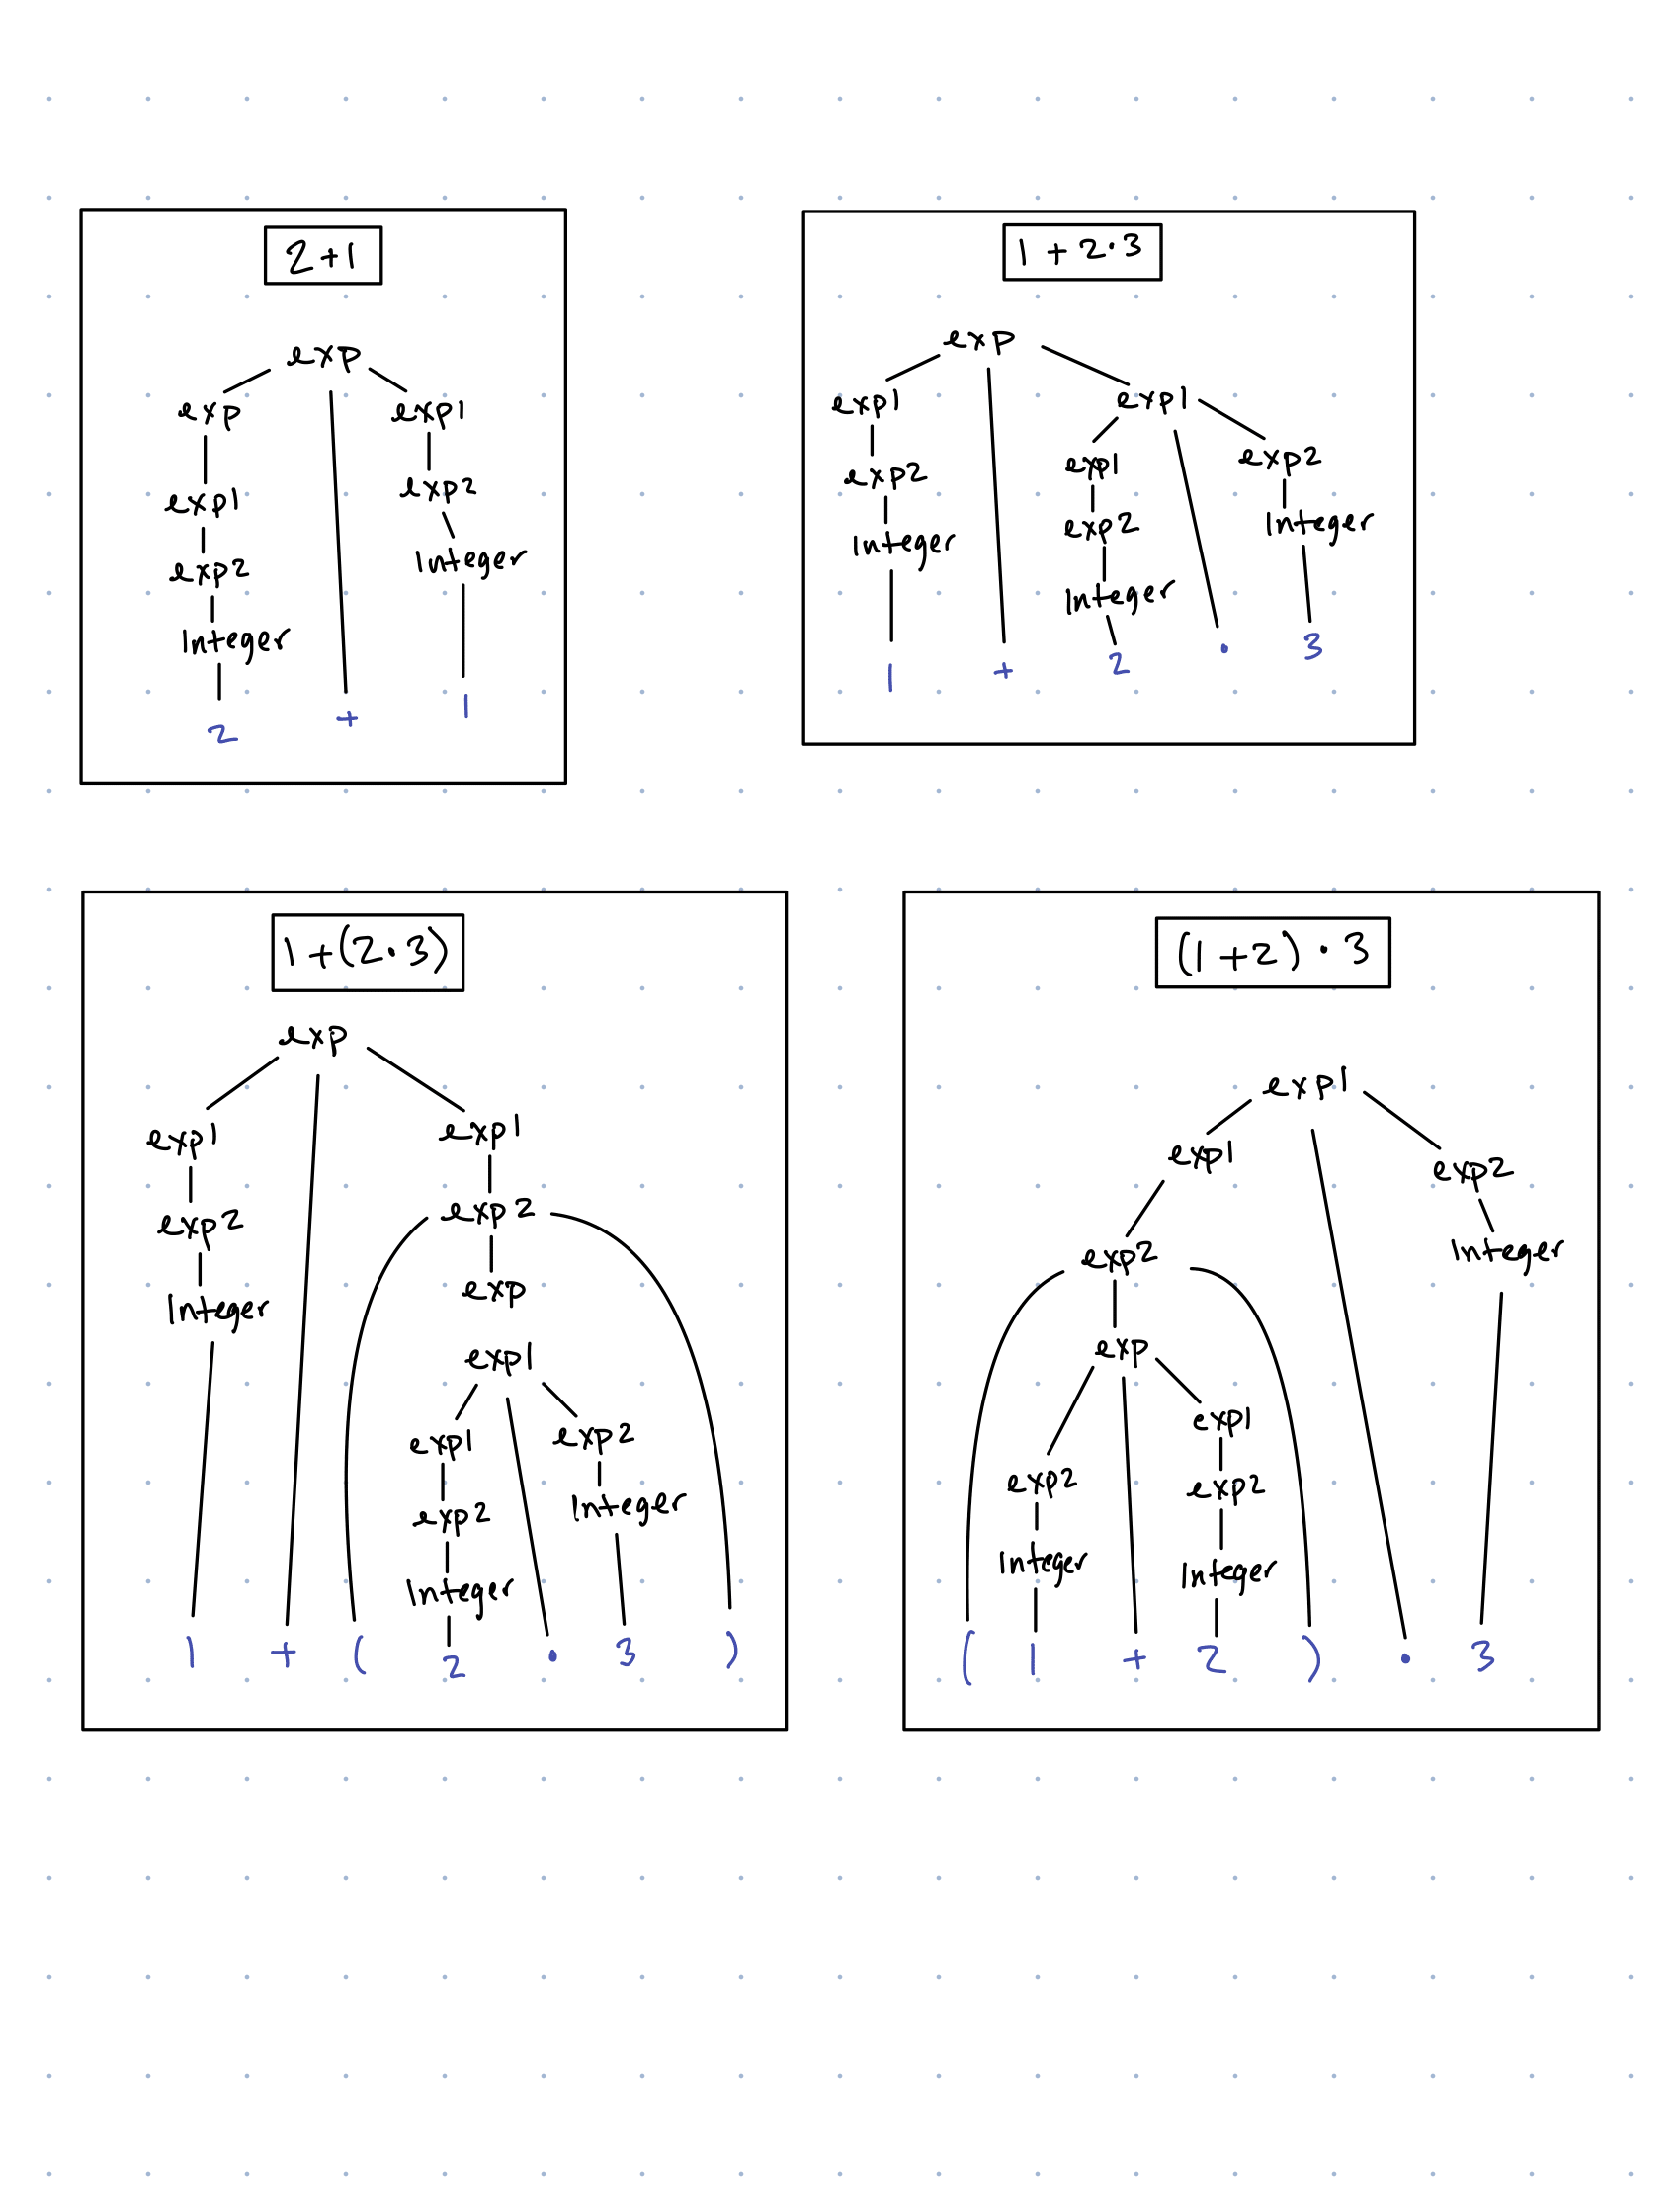
\includegraphics[scale=.5]{CPSC354 HW4-1.png}
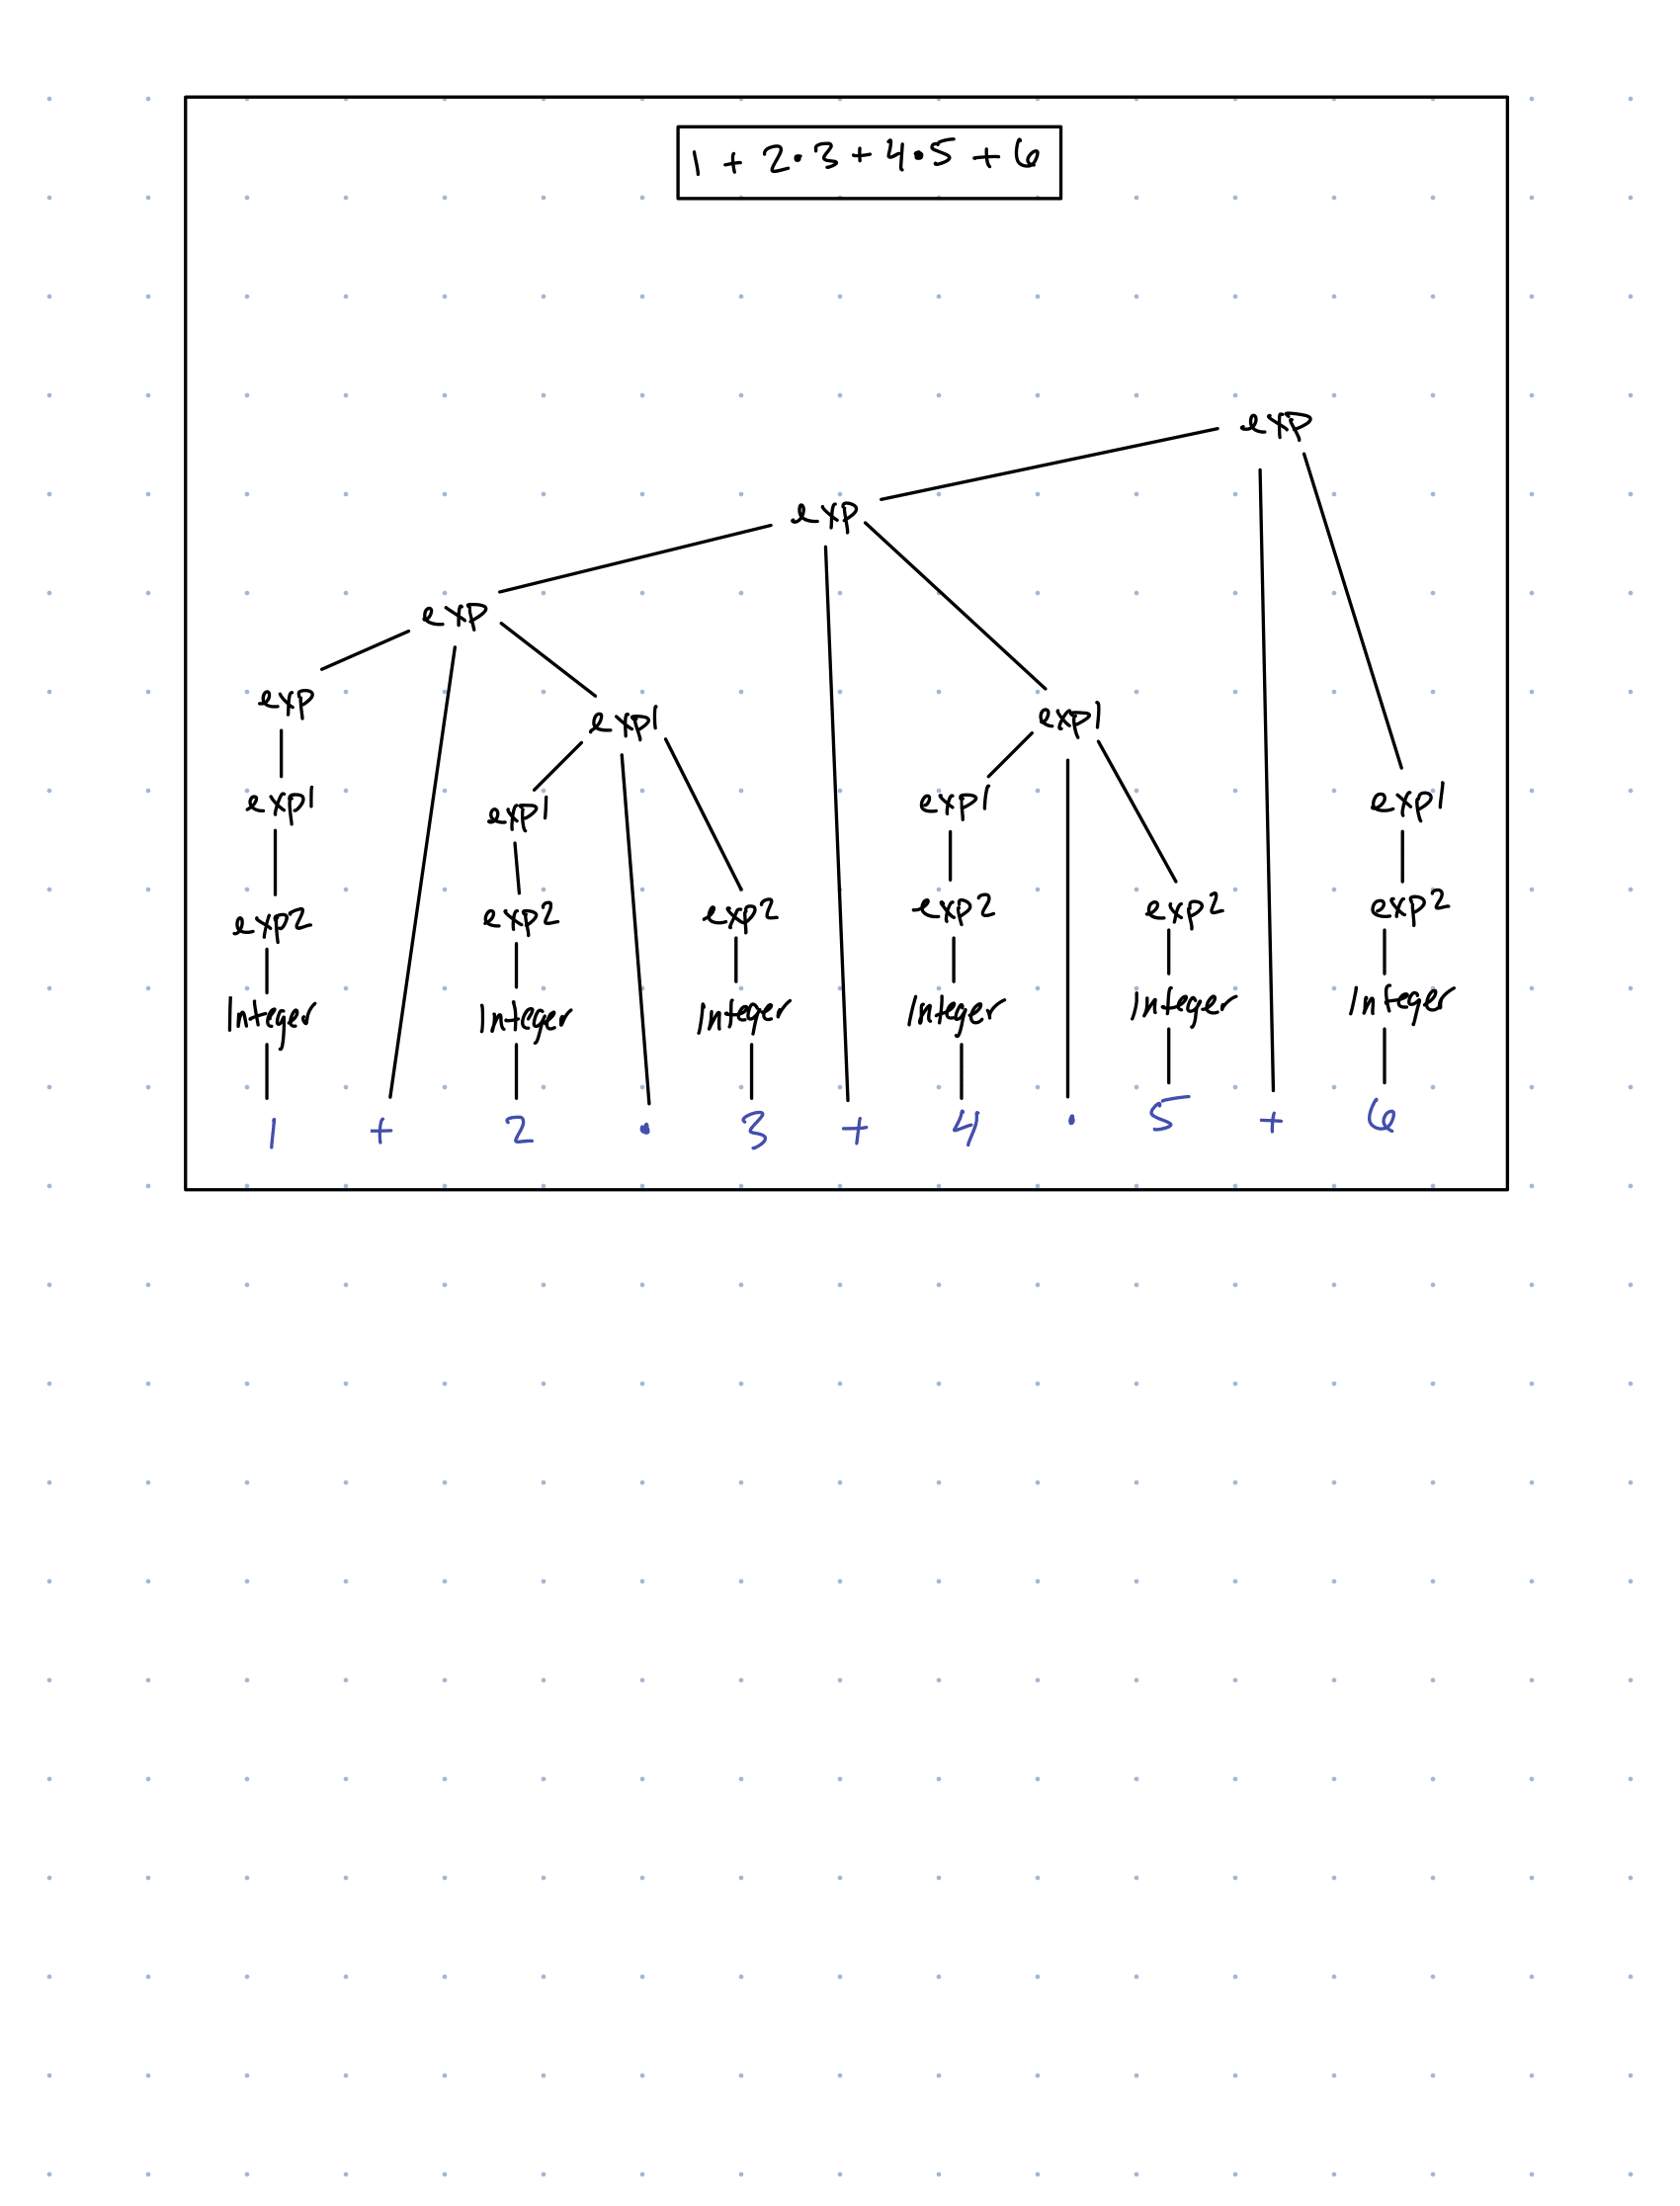
\includegraphics[scale=.6]{CPSC354 HW4-2.png}
\end{center}

\section{Lessons from the Assignments}

(Delete and Replace): Write three pages about your individual contributions to the project.

On 3 pages you describe lessons you learned from the project. Be as technical and detailed as possible. Particularly valuable are \emph{interesting} examples where you connect concrete technical details with \emph{interesting} general observations or where the theory discussed in the lectures helped with the design or implementation of the project.

Write this section during the semester. This is approximately a quarter of apage per week and the material should come from the work you do anyway. Just keep your eyes open for interesting lessons.

Make sure that you use \LaTeX{} to structure your writing (eg by using subsections).

\section{Conclusion}\label{conclusion}

(Delete and Replace): (approx 400 words) A critical reflection on the content of the course. Step back from the technical details. How does the course fit into the wider world of software engineering? What did you find most interesting or useful? What improvements would you suggest?

\begin{thebibliography}{99}
\bibitem[BLA]{bla} Author, \href{https://en.wikipedia.org/wiki/LaTeX}{Title}, Publisher, Year.
\end{thebibliography}

\end{document}
